\title{Study Guide 2 for Algebra-Based Physics-1: Mechanics (PHYS135A-01)}
\author{Dr. Jordan Hanson - Whittier College Dept. of Physics and Astronomy}
\date{October 24th, 2018}
\documentclass[10pt]{article}
\usepackage[a4paper, total={18cm, 27cm}]{geometry}
\usepackage{outlines}
\usepackage[sfdefault]{FiraSans}
\usepackage{graphicx}

\begin{document}
\maketitle

\section{Equations}
\begin{itemize}
\item Newton's First Law: $\vec{F}_{Net} = 0$ if $\vec{v}$ is constant.  Newton's Second Law: $\vec{F}_{Net} = m \vec{a}$. Newton's Third Law: $\vec{F}_{AB} = -\vec{F}_{BA}$.
\item Normal force: $\vec{N} = +mg\hat{y}$, if weight is $w = -mg\hat{y}$ (flat surface).
\item Force of Friction: $\vec{F} = -\mu \vec{N}$ (minus sign: opposes motion).
\item Static versus kinetic friction: $\mu_s \geq \mu_k$.
\end{itemize}

\section{Newton's Laws}
\begin{enumerate}
\small
\item An swimmer sinks at constant velocity to the bottom of the ocean near the shore.  The swimmer has a weight force downwards.  In which direction is there another force on the swimmer?
\begin{itemize}
\item A: Upwards.
\item B: Downwards.
\item C: Towards the shore.
\item D: Away from shore.
\end{itemize}
\item A soccer player in training begins to sprint down the field.  She has a mass $m$, is wearing a harness than has mass $M$, and has acceleration $a$.  If she exerts constant force through her cleats on the turf, and drops the harness, which of the following is true?
\begin{itemize}
\item A: Her new acceleration will be less than $a$.
\item B: Her new acceleration will be greater than $a$.
\item C: Her new acceleration will be equal to $a$.
\item D: Her new acceleration will be 0.
\end{itemize}
\item Consider Fig. \ref{fig:fbd1}.  Which of the following is true regarding the system in the diagram?
\begin{itemize}
\item A: It has no net force.
\item B: It is accelerating to the left.
\item C: It is accelerating to the right.
\item D: It is accelerating downwards. 
\end{itemize}
\begin{figure}[h]
\centering
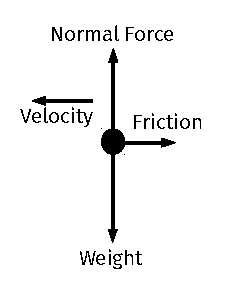
\includegraphics[width=0.15\textwidth]{figures/FBD3.pdf}
\caption{\label{fig:fbd1} A free body diagram for a system.}
\end{figure}
\clearpage
\item Consider Fig. \ref{fig:fbd1}.  Suppose the system reaches a point where there is no longer friction.  Which of the following is true?
\begin{itemize}
\item A: The system will move at a constant velocity.
\item B: The system will accelerate to the right.
\item C: The system will stop moving.
\item D: The system will accelerate to the left.
\end{itemize}
\item A 70 kg sprinter begins a run at rest and reaches 10 m/s in 3.0 seconds.  What force does he exert on the track? \\ \vspace{2.0cm}
\item Consider Fig. \ref{fig:sled}, in which two children pull their friend on a sled resting on snow with forces $\vec{F}_1$ and $\vec{F}_2$.  (a) What is the magnitude of the net force (no friction)? (b) If sled and the child on it have total mass 40 kg, what is the acceleration? \\ \vspace{2.5cm}
\begin{figure}[h]
\centering
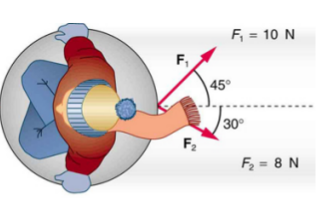
\includegraphics[width=0.4\textwidth]{figures/sled.png}
\caption{\label{fig:sled} Two children pull a third on a sled.}
\end{figure}
\item A 20,000 kg jet pushes through the air with a forward force of $10^6$ N, and faces air resistance equivalent to $5 \times 10^4$ N.  What is the acceleration of the jet? \\ \vspace{2cm}
\end{enumerate}
\section{Friction and Drag}
\small
\begin{enumerate}
\item A woman drags a piece of luggage across a floor.  If the mass of the luggage is 30 kg, and she exerts a force of 300 N, what is the coefficient of kinetic friction between the luggage and floor? \\ \vspace{1.5cm}
\item Consult Fig. \ref{fig:coeff}. (a) What is the magnitude of the force of friction exerted on an oiled steel piston experiencing a normal force of 10 N from another steel surface? (b) What would the result have been if the steel had no oil? \\ \vspace{1.5cm}
\begin{figure}
\centering
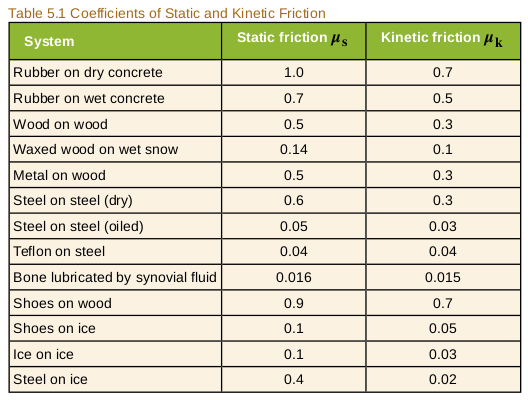
\includegraphics[width=0.55\textwidth]{figures/coefficients.png}
\caption{\label{fig:coeff} (Left) Frictional coefficients for exercise 2, \textbf{Friction and Drag}.}
\end{figure}
\item Consult Fig. \ref{fig:blocks}.  Recall the lab in which we measured the coefficient of static friction, $\mu_s$.  If $\mu_s = 0.5$, and $m_2=200$ grams, what is the largest mass $m_1$ can be before the system begins to accelerate? \vspace{1cm}
\begin{figure}[hb]
\centering
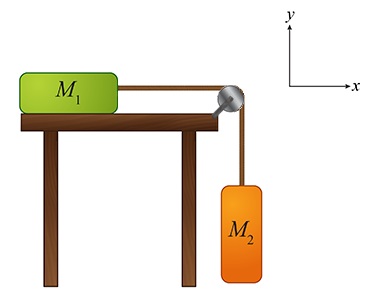
\includegraphics[width=0.25\textwidth]{figures/table.png}
\caption{\label{fig:blocks} Diagram for exercise 3, \textbf{Friction and Drag}.}
\end{figure}
\item A system travels at a \textit{terminal velocity} $v_{T} = \sqrt{2mg/C\rho A}$.  (a) What is $v_{T}$ for a falling system who with $m=200$ kg, $A=2$ m$^2$, $C \approx 0.4$, in air with $\rho_{air}=1.225$ kg/m$^3$? (See section 5.3 of the textbook).
\end{enumerate}
\end{document}